\chapter{User's Manual} \label{ch:manual}

This chapter will describe the usage and features of the \SB in detail and serve as a user's manual. 
\autoref{sec:manual-overview} will give an overview of the IEC editor and the process of creating the IEC project. 
\autoref{sec:manual-sdg} will cover the steps needed to use the \SB. A detailed description of the \SB features will be 
given in \autoref{sec:manual-features}. Finally \autoref{sec:manual-usecases} will cover each use case and include 
examples of problems that might be solved.


\section{Overview} \label{sec:manual-overview}

After first installing the \SB plugins and opening the \emph{\SB} perspective, the Eclipse workbench should look like 
\autoref{fig:manual-perspective}. On the left and right are the standard Eclipse Project Explorer and Outline views, 
respectively. On the bottom is the new \SB view, below the Project Explorer is the Instance Hierarchy view. Those two 
views can be opened in any other perspective using the \emph{Show View} dialog (Alt+Shift+Q, Q by default) as shown in 
\autoref{fig:manual-open_views}.

\begin{figure}[hp]
  \centering
    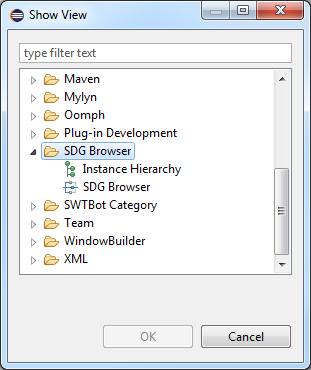
\includegraphics[scale=0.55]{bilder/manual-open_views}
  \caption{Entries in the \emph{Show View} dialog for the \SB views}
  \label{fig:manual-open_views}
\end{figure}

\begin{figure}[htp]
  \centering
    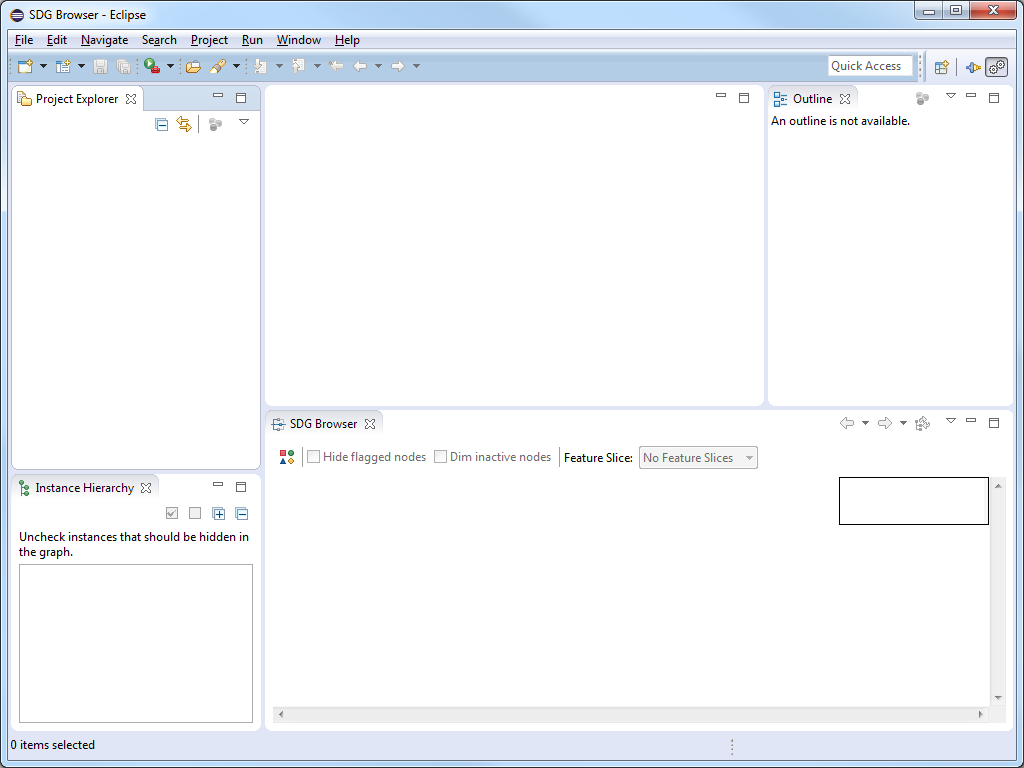
\includegraphics[width=\textwidth]{bilder/manual-perspective}
  \caption{Default layout of the \emph{\SB} perspective}
  \label{fig:manual-perspective}
\end{figure}

In order to use the \SB with IEC source code, you first need to build it in IecEdit and import it as an Eclipse IEC 
Project. A project also needs to be rebuilt in IecEdit whenever it is moved to a different location.

\begin{enumerate}
  \item Create a new Eclipse project and select \emph{IEC Project} from the IEC category (see 
  \autoref{fig:manual-new_project1}).
  
  \item On the next page, enter a name for the project and select the location of the IEC project files 
  (\autoref{fig:manual-new_project2}). This is the location where the Eclipse project file will be created, the IEC 
  source code may be located there or in any subdirectory.
  
  \item In case you have a standard project layout with HMI, the default source code locations may be used 
  (\texttt{/prj/Source/IMM/ieccontrol} for IEC code and \texttt{/prj/Source/IMM/view/viewKVS} for view code). 
  Otherwise, uncheck the checkbox and specify the paths (relative to the project location selected earlier). If you 
  don't have HMI code, leave that text box empty.
\end{enumerate}

\begin{figure}[hp]
  \centering
    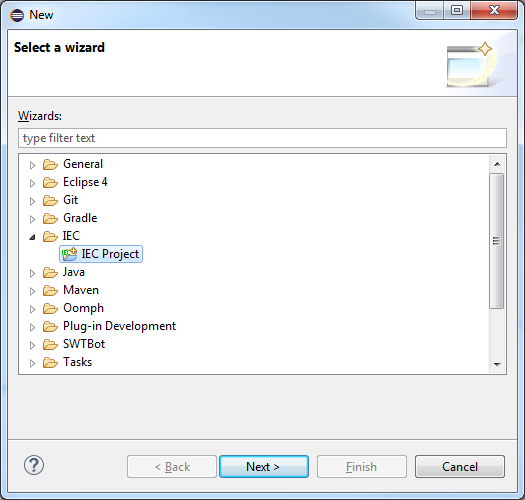
\includegraphics[scale=0.55]{bilder/manual-new_project1}
  \caption{Create a new IEC project\ldots}
  \label{fig:manual-new_project1}
\end{figure}

\begin{figure}[hp]
\centering
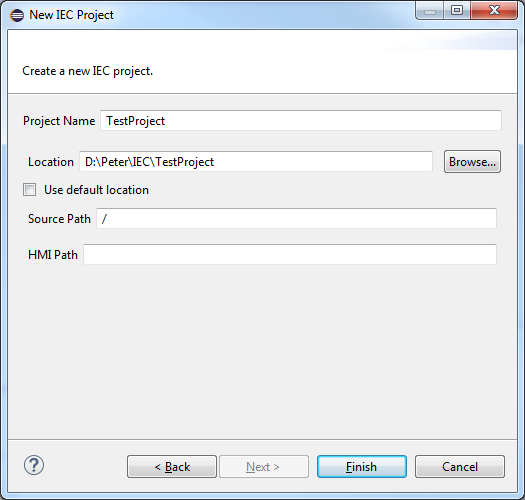
\includegraphics[scale=0.55]{bilder/manual-new_project2}
\caption{\ldots{}and specify the source code location}
\label{fig:manual-new_project2}
\end{figure}

After the project has been created, the Project Explorer will show all files and folders under the project directory, 
with some exceptions. Files recognized by any Eclipse editor can be opened directly, including IEC source files. Note, 
however, that the IEC editor as it's currently implemented doesn't allow editing. This is so files containing Keba's 
proprietary representation of the source code (the so called \emph{UFF code}), in addition to the textual IEC code, 
don't get corrupted.

By default, IEC binaries and files related to Keba's IecEdit will not be shown in the Project Explorer. This may be 
changed by disabling the respective filters in the Project Explorer (via the \emph{Customize View...}\ menu item).

\autoref{fig:manual-editor} shows an IEC file opened in the Eclipse editor. Note the file outline on the right hand 
side. The IEC editor shows only the textual IEC code, the UFF code is truncated from the output.

The IEC editor allows navigation through the IEC code in a number of ways.

\begin{itemize}
  \item The outline view can be used to navigate within a file to different procedures or declarations of variables.
  
  \item The editor also supports hyperlinks which may be used to go to the definition of a variable or procedure (via 
  Ctrl+Click on the name).
  
  \item Furthermore, searching for all references to a particular source code element in the whole project is 
  implemented as well. This can be accessed in the Eclipse \emph{Search} menu or via the editor context menu 
  (\autoref{fig:manual-search}, \autopageref{fig:manual-search}).
\end{itemize}

\begin{figure}[hp]
  \centering
    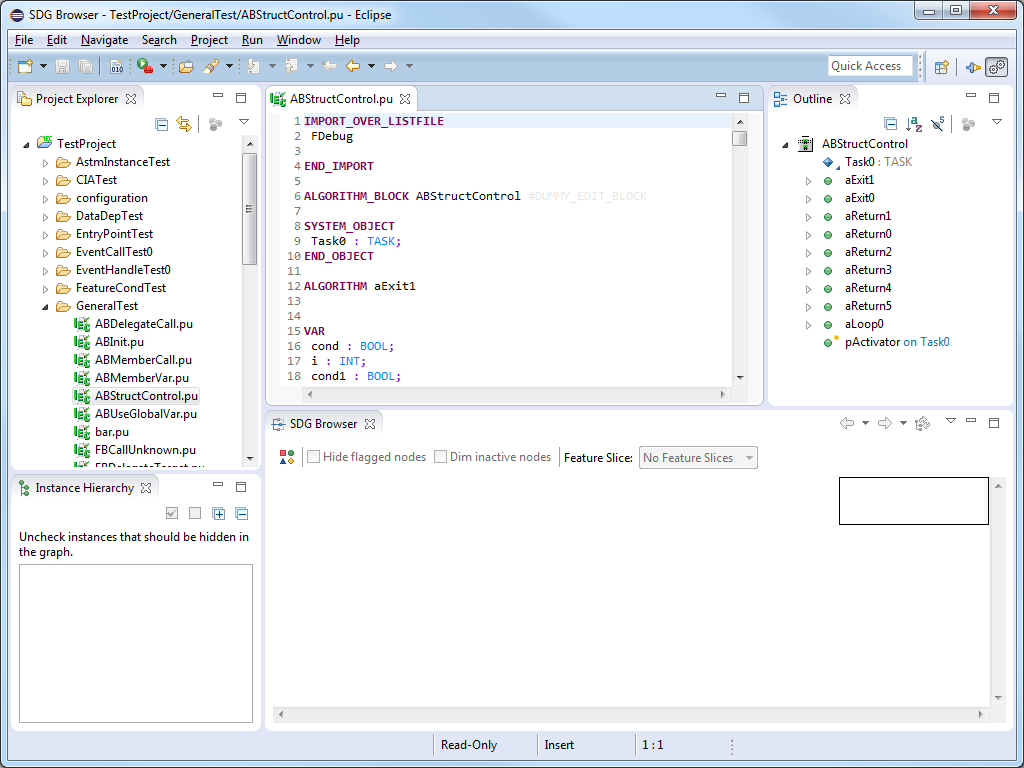
\includegraphics[width=\textwidth]{bilder/manual-editor}
  \caption{IEC file opened in Eclipse, an outline of the file is shown to the right}
  \label{fig:manual-editor}
\end{figure}


\section{Using the SDG} \label{sec:manual-sdg}

Everything shown so far works without manually building the Eclipse project, since the source code is automatically 
parsed once any of the project's files are opened. However, the SDG must be built before the \SB can be used. For large 
projects this can take several minutes.

To build the SDG, open any file within the project and then hit Ctrl+B or select \emph{Build Project} from the 
\emph{Project} menu (\autoref{fig:manual-build1}). If you try to use any of the \SB operations before the project has 
been built, you will be asked whether you want to build the project (\autoref{fig:manual-build2}).

\begin{figure}[hp]
  \centering
    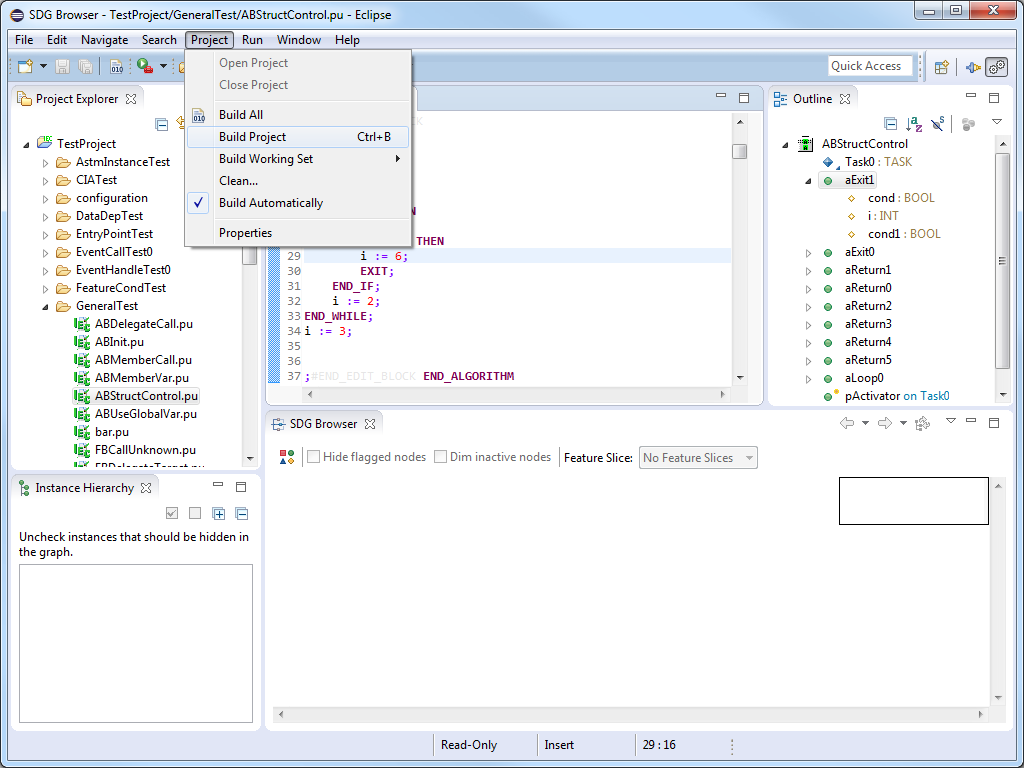
\includegraphics[width=\textwidth]{bilder/manual-build1}
  \caption{Building the IEC project before using \SB operations}
  \label{fig:manual-build1}
\end{figure}

\begin{figure}[hp]
  \centering
    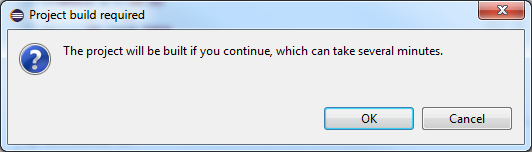
\includegraphics[scale=0.55]{bilder/manual-build2}
  \caption{Confirmation before starting a lengthy project build}
  \label{fig:manual-build2}
\end{figure}

\clearpage
The \SB operations can be accessed from the IEC editor context menu (see \autoref{fig:manual-editor_context}). Usually 
you would select a source code element of interest (variable, statement, procedure) in the editor and then choose the 
desired operation from the context menu. In case nothing is selected, the whole line will be selected automatically for 
convenience.

\begin{figure}[hp]
  \centering
    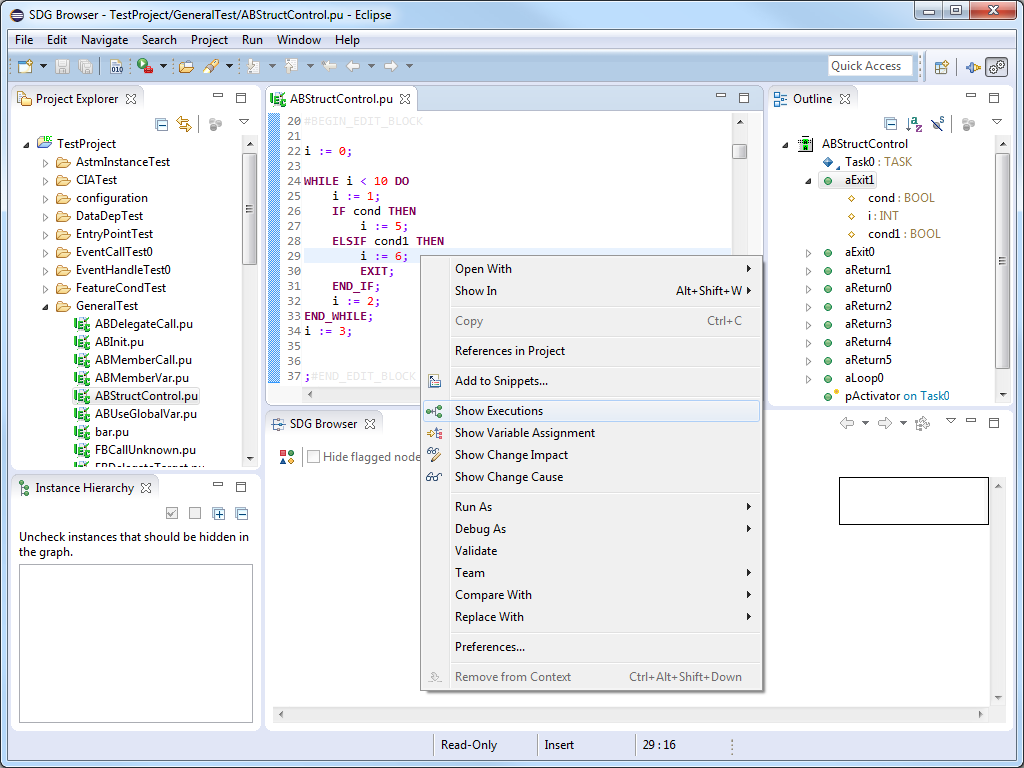
\includegraphics[width=\textwidth]{bilder/manual-editor_context}
  \caption{IEC editor context menu entries for \SB operations}
  \label{fig:manual-editor_context}
\end{figure}

\autoref{fig:manual-executions1} shows the screen after choosing \emph{Show Executions} from the context menu. Notice 
the whole statement is selected now. The \SB view shows a node for the selected statement \lstinline|i := 6|, and nodes 
for all immediate predecessors (only \lstinline|cond1| int his case). The nodes are contained by a node that represents 
the procedure those statements belong to (the algorithm \lstinline|aExit1|).

\begin{figure}[htp]
  \centering
    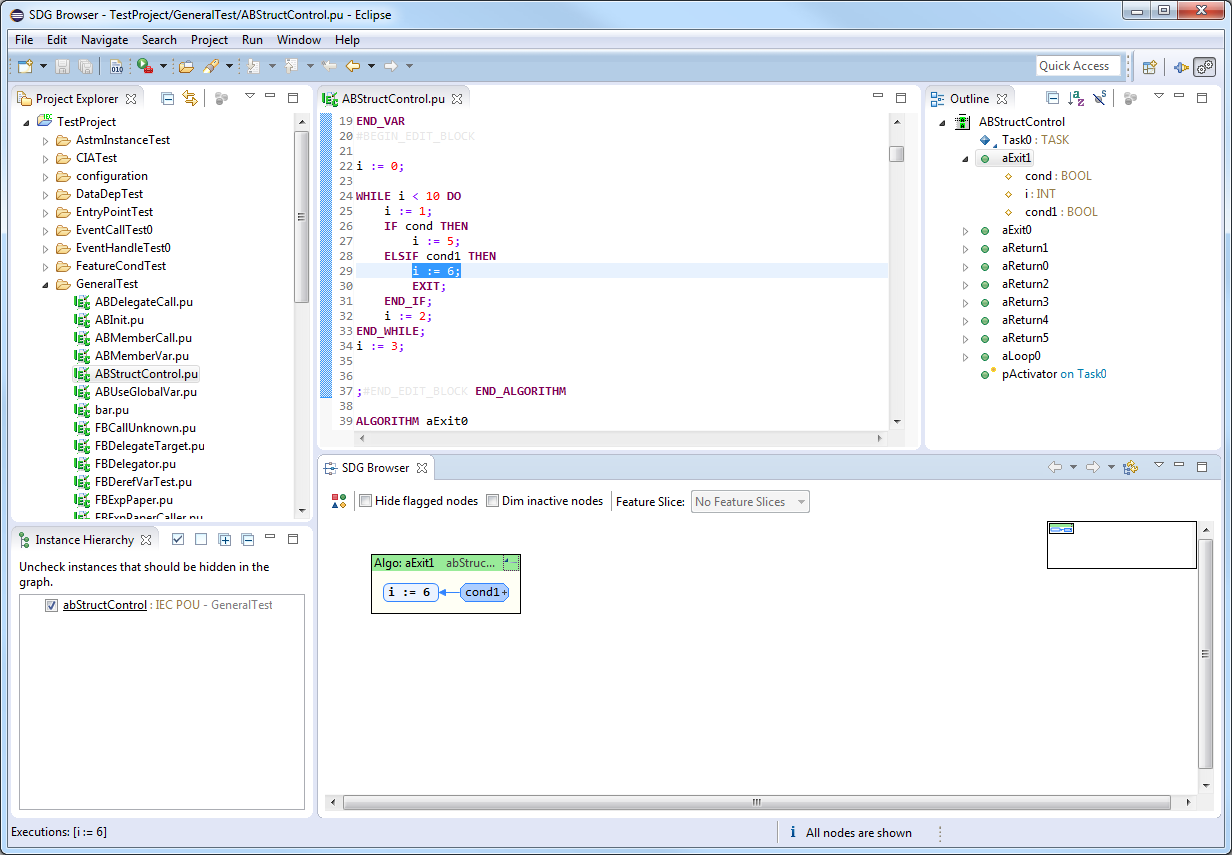
\includegraphics[width=\textwidth]{bilder/manual-executions1}
  \caption{Screen after choosing an \SB operation}
  \label{fig:manual-executions1}
\end{figure}

You can navigate by panning the view: click and then drag with the middle mouse button anywhere in the graph. At the 
top right corner of the \SB view you can see an overview thumbnail that shows the whole graph. This can also be used to 
navigate large graphs: click anywhere in the thumbnail to center the view around that point.

The \SB includes a legend as a quick reference of what the different colors and shapes of nodes and edges represent. 
Click on the leftmost icon in the toolbar of the \SB view to show/hide it (see \autoref{fig:manual-legend}).

\begin{figure}[hp]
  \centering
    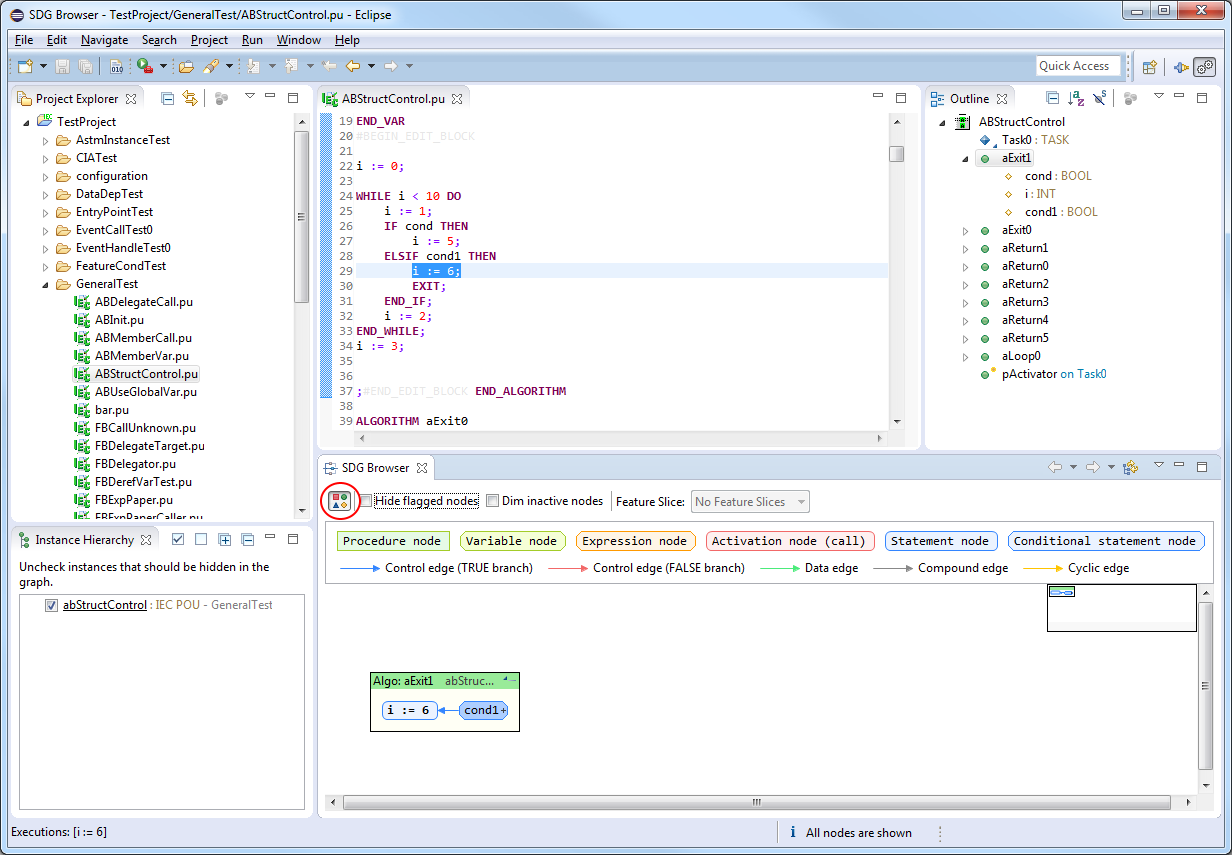
\includegraphics[width=\textwidth]{bilder/manual-legend}
  \caption{A legend shows different node and edge types}
  \label{fig:manual-legend}
\end{figure}

For details on the types of nodes and edges in the SDG, as well as its structure, refer to \autoref{ch:sdg}. There are 
the following types of nodes in the SDG.

\begin{itemize}
  \item Procedure nodes represent executable procedures like functions, event handlers, process algorithms, etc. 
  Procedure nodes may also be containers of the statements and variables within.
  
  \item Variable nodes represent all kinds of variables: local, global, and member variables, formal parameters and 
  return values.
  
  \item Expression nodes represent actual parameter expressions.
  
  \item Activation nodes represent calls, as well as other kinds of activation (for example, setting an event will 
  cause all its event handlers to be executed, but this is not a call in the traditional sense).
  
  \item Statement nodes and conditional statement nodes represent ordinary and conditional statements, respectively.
\end{itemize}

The SDG may contain two types of edges, two additional kinds are introduced by the \SB.

\begin{itemize}
  \item Control edges represent a control dependency, the target node will only be executed if the source node is as 
  well. In case the source node is a conditional statement, the edge color will indicate whether the target node is 
  executed if the condition is true or false.
  
  \item Data edges represent a data flow from the source node (e.g.\ a write to a variable) to the target node (e.g.\ a 
  read from a variable).
  
  \item Compound edges between container nodes indicate more than one edge.
  
  \item A cyclic edge indicates an edge that introduces a cycle in the graph, it always leads to a node that has 
  already been discovered earlier.
\end{itemize}

You will have noticed that the node for the conditional statement \lstinline|cond1| is of a darker shade than the 
statement node (and shows a plus sign on its right side). This means that it can be expanded to reveal nodes connecting 
to it. Click on the node to expand it, the result should look like \autoref{fig:manual-executions2}.

\begin{figure}[hp]
  \centering
    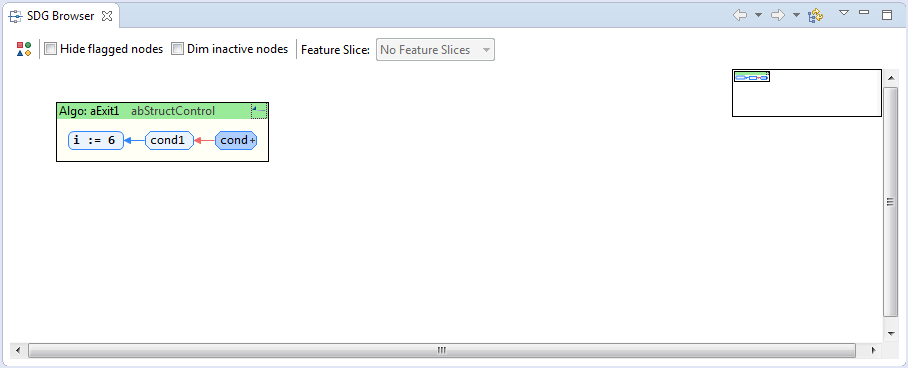
\includegraphics[width=\textwidth]{bilder/manual-executions2}
  \caption{Nodes that can be expanded are of a darker shade and marked by a little plus sign on their right side}
  \label{fig:manual-executions2}
\end{figure}

After expanding all nodes, the graph should look like \autoref{fig:manual-executions3}. Notice that there are now two 
procedures involved, algorithm \lstinline|aExit1| is called by algorithm \lstinline|pActivator|, which is in turn 
called by the artificial \lstinline|main| procedure. You can ignore the artificial main procedure most of the time, 
it's just an artifact of the analysis. In this case it signals that \lstinline|pActivator| is an entry point of the 
program (all entry points are called by \lstinline|main|).

\begin{figure}[hp]
  \centering
    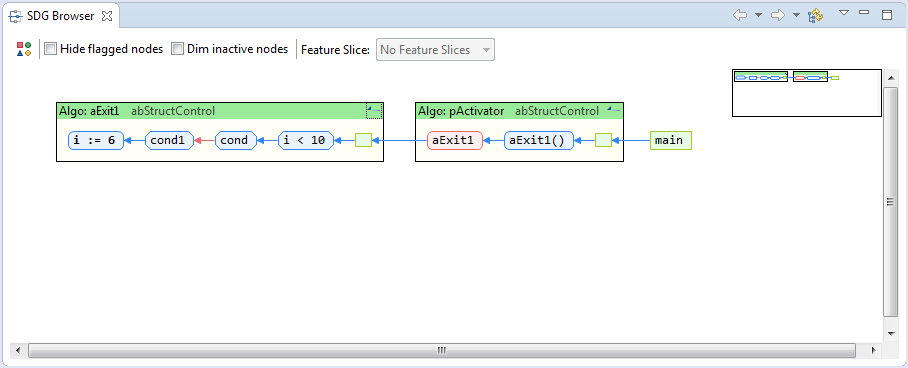
\includegraphics[width=\textwidth]{bilder/manual-executions3}
  \caption{This graph shows one procedure calling another, the main procedure signals an entry point.
    Notice the small nodes, which represent the procedure they are contained in.}
  \label{fig:manual-executions3}
\end{figure}


\section{Additional Features} \label{sec:manual-features}

There are a number of additional feature which may prove helpful, especially when working with larger graphs.

Hovering over a node or edge opens a tooltip, which shows some additional information about the element (see 
\autoref{fig:manual-tooltip} for an example). For nodes of large statements (which are truncated so the node doesn't 
get too large) the tooltip also contains the entire statement.

\begin{figure}[hp]
  \centering
    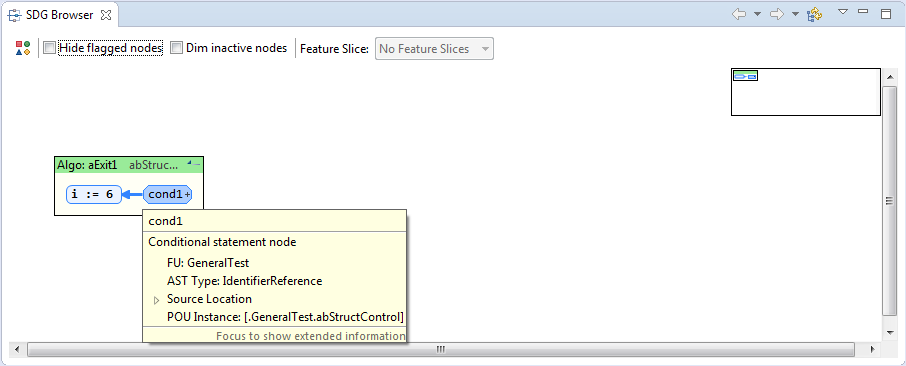
\includegraphics[width=\textwidth]{bilder/manual-tooltip}
  \caption{Tooltips provide further information about nodes and edges}
  \label{fig:manual-tooltip}
\end{figure}

Right clicking on a node opens a context menu as seen in \autoref{fig:manual-node_context},which contains several 
additional actions.

\begin{description}
  \item[Highlight Edges] highlights all edges connected to the node. This may be   helpful for following long edges 
  that don't fit on the screen.
  
  \item[Show Source] opens the source code location associated with the node in the IEC editor, if possible 
  (\autoref{fig:manual-show_source}. Note that not all nodes may have a source location associated with them. This can 
  also be invoked by clicking on a node while holding the control key.
  
  \item[Show Instance Declaration] opens the source code location defining the object instance the node belongs to.
  
  \item[Set/Remove Flag] sets or removes the node flag (\autoref{fig:manual-flag}). Flagged nodes may be hidden by 
  activating the corresponding checkbox (see \autoref{fig:manual-hide_flagged}).
  
  \item[Collapse All] collapses a node and all its successors at once. Note that this is different from simply 
  collapsing a node, in which case the expansion state of all its predecessors is preserved.
  
  \item[Expand Next Level] expands all successors of the node.
\end{description}

The context menu also provides entries for executing a use case on the node.

\begin{figure}[p]
  \centering
    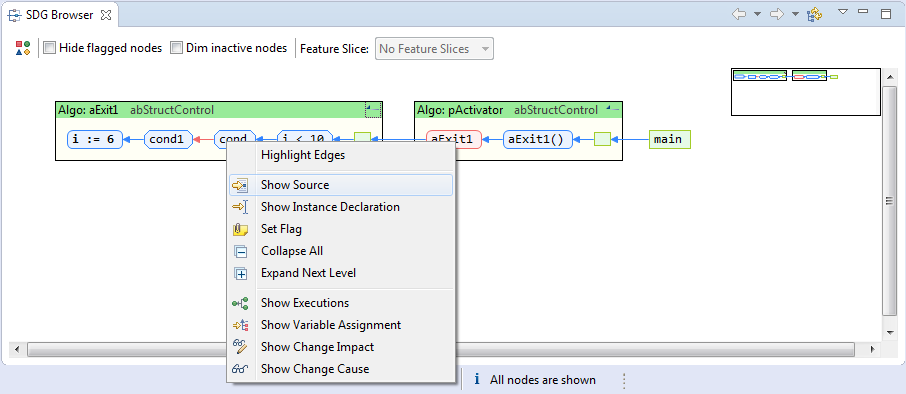
\includegraphics[width=\textwidth]{bilder/manual-node_context}
  \caption{A context menu provides actions on nodes}
  \label{fig:manual-node_context}
\end{figure}

\begin{figure}[p]
  \centering
    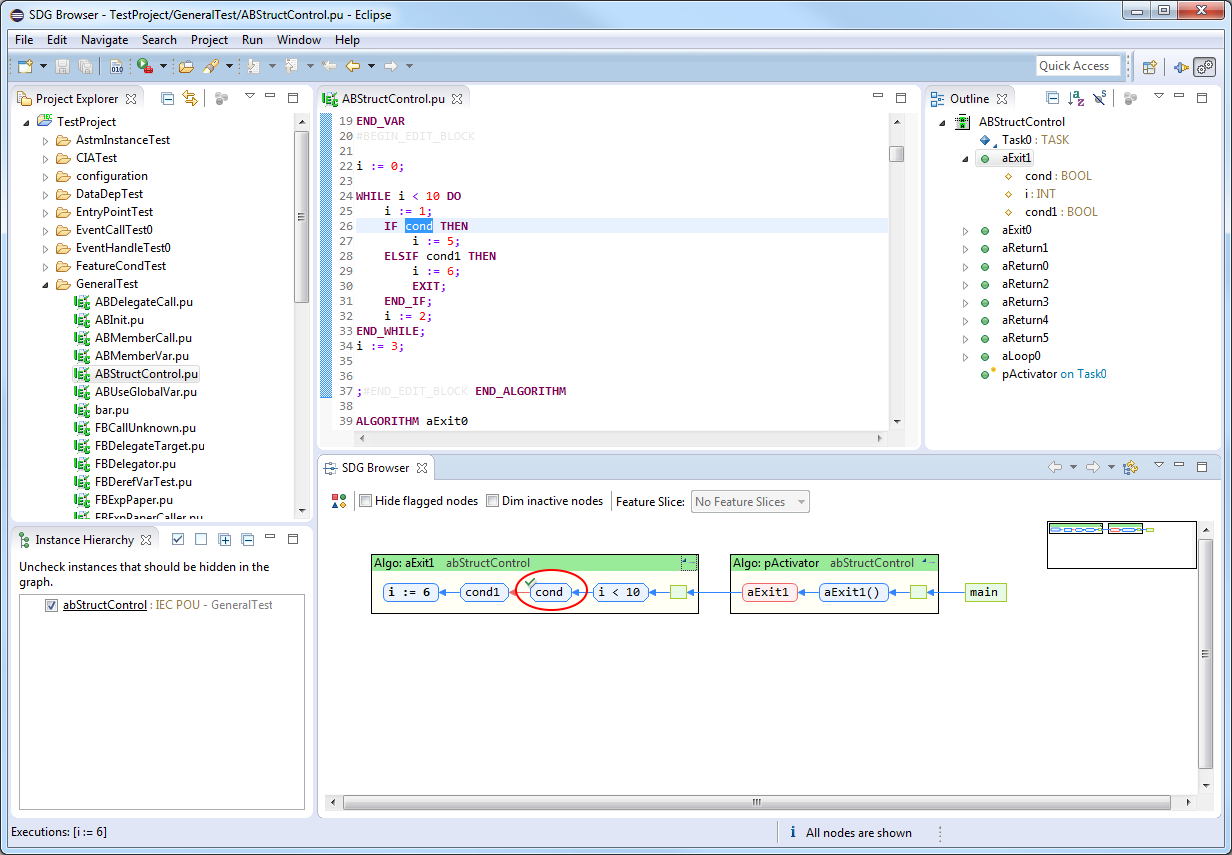
\includegraphics[width=\textwidth]{bilder/manual-flag}
  \caption{Alt+Click on a node to set/remove its flag}
  \label{fig:manual-flag}
\end{figure}

\begin{figure}[p]
  \centering
    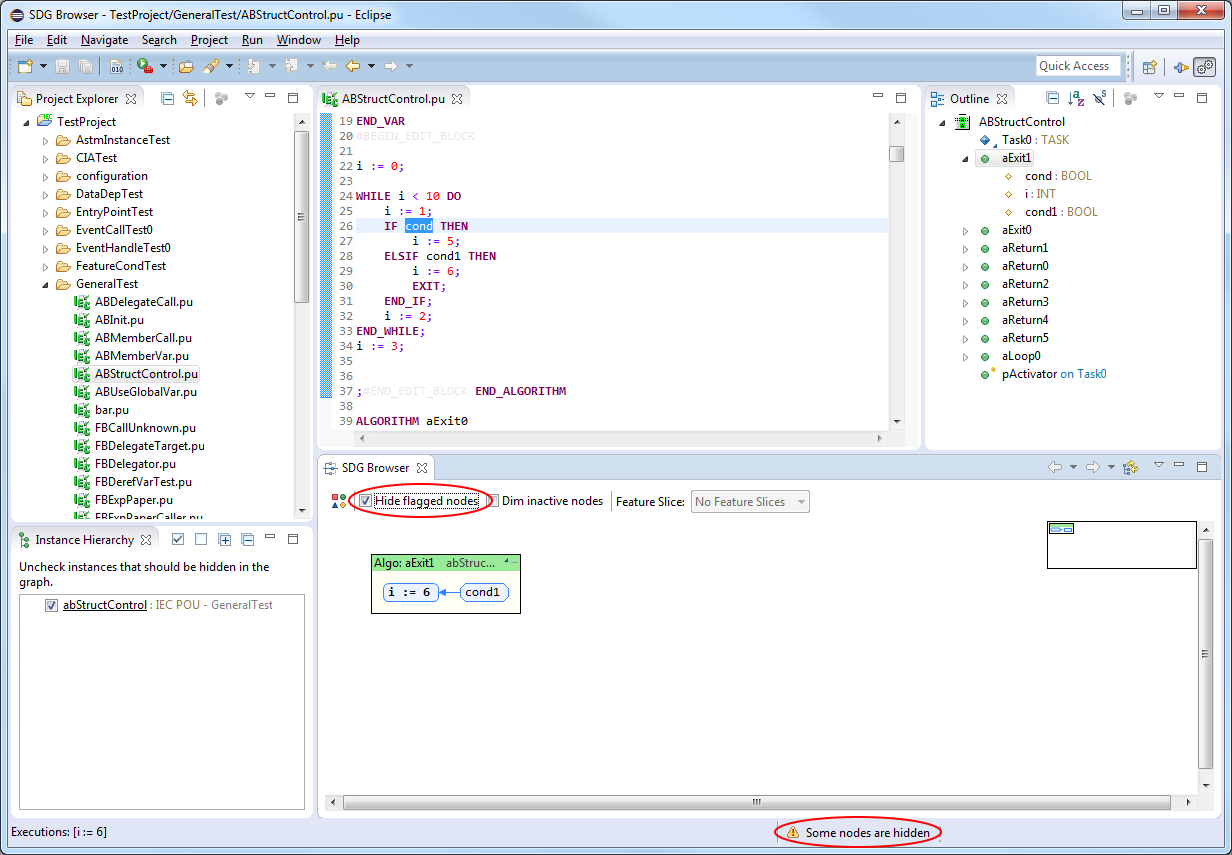
\includegraphics[width=\textwidth]{bilder/manual-hide_flagged}
  \caption{Flagged nodes can be hidden to reduce visual clutter}
  \label{fig:manual-hide_flagged}
\end{figure}

\begin{figure}[p]
  \centering
    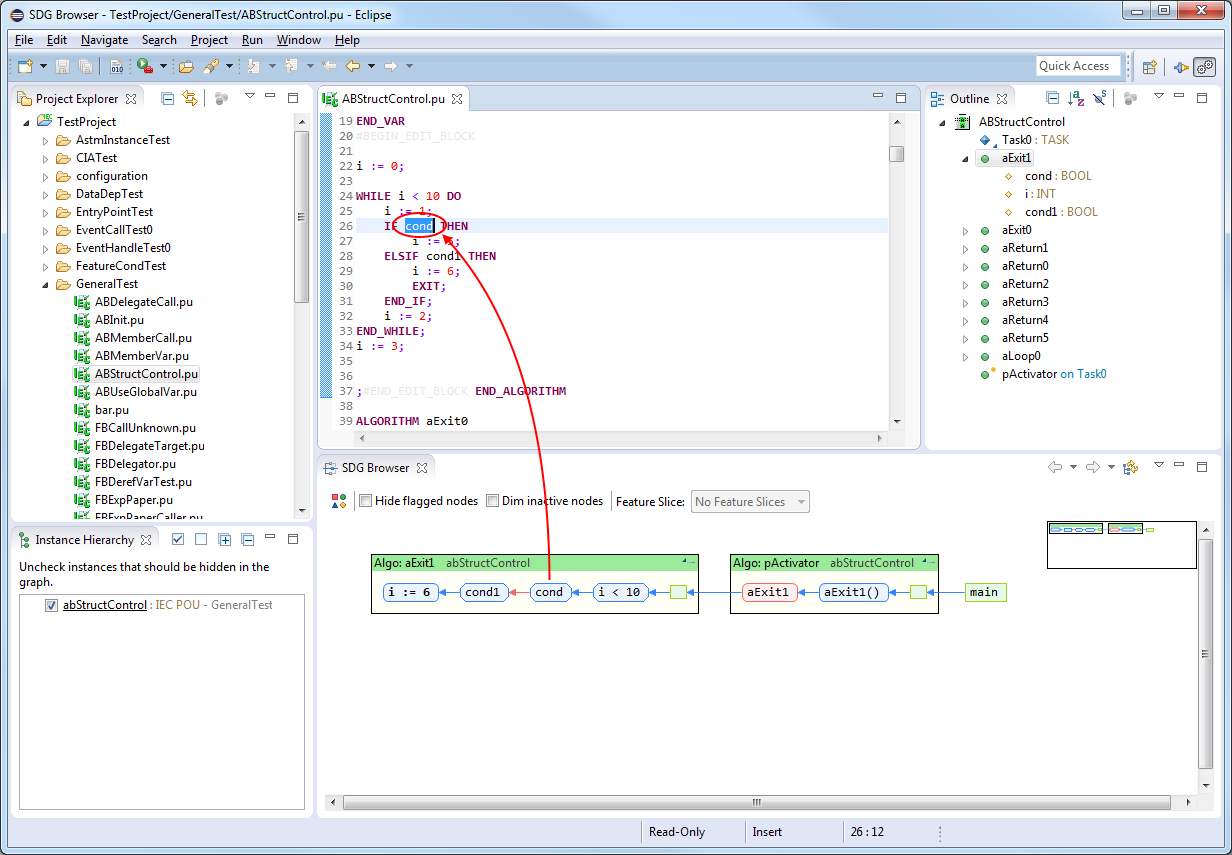
\includegraphics[width=\textwidth]{bilder/manual-show_source}
  \caption{Navigation from SDG nodes to their source code is easily accessible (Ctrl+Click on a node, or from the 
    context menu)}
  \label{fig:manual-show_source}
\end{figure}

\begin{figure}[p]
  \centering
    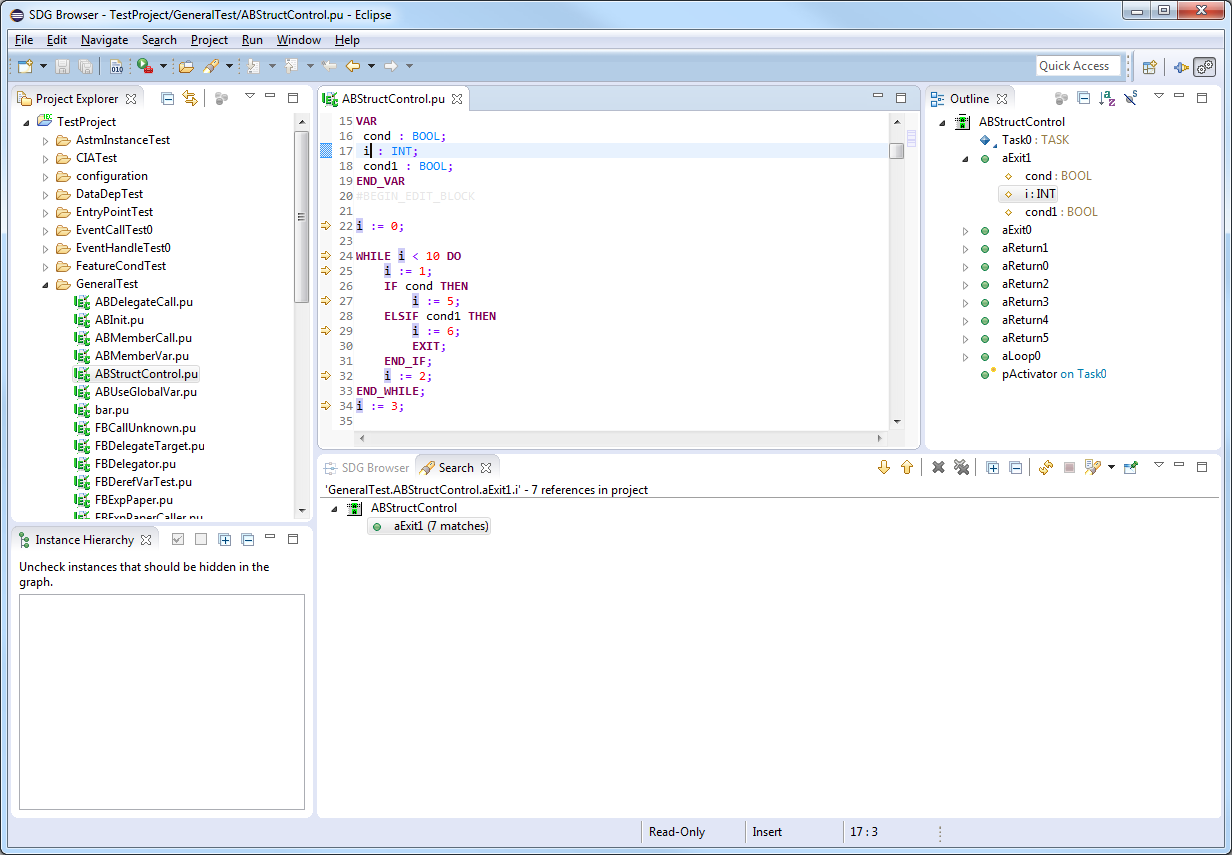
\includegraphics[width=\textwidth]{bilder/manual-search}
  \caption{Search results for a local variable using \emph{References in Project}}
  \label{fig:manual-search}
\end{figure}

% TODO Maybe mention pruning


\section{Use Cases} \label{sec:manual-usecases}

TODO
